\documentclass[12pt]{article}

\usepackage[utf8]{inputenc}
\usepackage{mhchem}
\usepackage{chemfig}
\usepackage{fancyhdr}
\usepackage{grapicx}

\title{Kemiaflevering 14}
\author{Jeppe Møldrup}
\date{}

\pagestyle{fancy}
\fancyhead[L]{Jeppe Møldrup}
\fancyhead[C]{Kemi 14}
\fancyhead[R]{08/04-2019}

\begin{document}

\maketitle{}

\section*{Opgave 1}

a.

\chemfig{*6(-(-[-2]-[-1]OH)---(-(-[3])-[1])--)}

b.

Carbonylgruppe i den første\\
Alkoholgruppe i den anden\\
Carboxylsyregruppe i den sidste\\

c.

ud fra testen kan man se at nummer 3 og 1 reagerer med brom, og derfor må have dobbeltbindinger mellem carbon.
Og nummer 4 er den eneste der reagerer i hydrazin-testen. Så derfor må 4 indeholde en carbonylgruppe, dvs. det må være menthon.
Nummer 3 og 1 Må begge enten være terpinen eller elemen idet de begge reagerer i bromtesten. Og så ved udelukkelse må nummer 2 være hexansyre.

For at skeldne mellem nummer 3 og 1 kunne man kigge efter OH-strækninger i phenol der vil være omkring 3100-3600 $cm^-1$ og kun ville
være i IR-plottet for terpinen.

\section*{Opgave 2}

a.

\schemestart
\chemfig{cl-[-2](-[0])(-[4])-[-2]} \arrow{->} \chemfig{-[-2](-[-3])=[-1]} \+ \ce{Cl}
\schemestop

b.

Gibbs fri energi er givet ved formlen

$$\Delta G^{\circ} = \Delta H^{\circ} - T \cdot \Delta S^{\circ}$$

Så jeg laver lineær regression på dataet og får

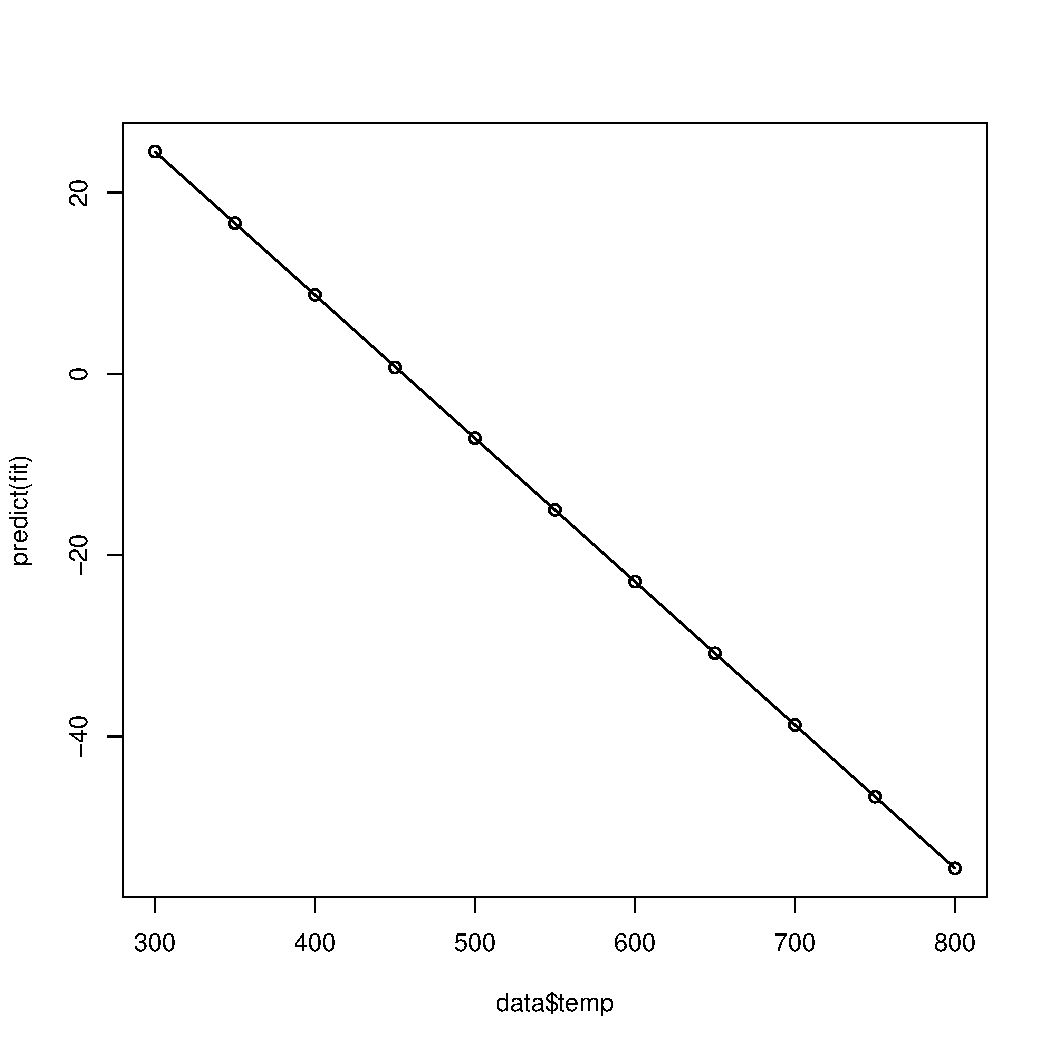
\includegraphics[width=\textwidth]{kemi1.pdf}

med funktionen
$$\Delta G^{\circ} = 71.97 \ kJ\cdot mol^-1 - T \cdot 15.82 \ kJ\cdot mol^-1 \cdot K^-1$$
Hvor $\Delta H^{\circ}$ så er $71.97 \ kJ\cdot mol^-1$

c.

Ændringen i fri gibbs energi skal være negativ for at en reaktion kan forløbe spontant.
Så idet funktionen er aftagende, finder jeg punktet hvor funktionen skærer x-aksen og dermed
bliver negativ
$$solve(0 = 71.97-T\cdot 15.82,T) \rightarrow T = 455.04 \ K$$
Som svarer til omkring 181.9 grader celsius.

d.

Jeg ved at K afhænger af gibbs energi i formlen
$$-\Delta G^{\circ} = R\cdot T\cdot ln K$$
Så jeg finder først gibbs energi ved $260^{\circ} = 533.15\ K$ med formlen fra b
$$-\Delta G^{\circ}(533.15\ K) = 12.35\ kJ\cdot mol^-1$$
Så isolerer jeg K
$$-\Delta G^{\circ} = R\cdot T\cdot ln K \Leftrightarrow K = e^{\frac{-\Delta G^{\circ}}{R\cdot T}}$$
Og indsætter
$$K = e^{\frac{12.35\ kJ\cdot mol^-1}{8.314\cdot 533.15}} = 16.21$$
K er enhedsløs idet $R\cdot T$ har samme enhed som gibbs energi og derfor går de to ud med hinanden.

e.

Idealgasligningen er givet ved
$$pV = nRT$$
Jeg kender alle værdier deri undtagen $n$, så jeg isolerer
$$n = \frac{pV}{RT}$$
Så indsætter jeg
$$n = \frac{0.52\ bar \cdot 3\ L}{0.08314472\ L\cdot bar\cdot mol^-1\cdot K^-1\cdot 533.15\ K} = 0.0352\ mol$$
Jeg antager at alt 2-chlor-2-methylpropan er omdannet til 2-methylprop-1-en. og derfor vil der før reaktionen have været 0.0352 mol
2-chlor-2-methylpropan. Så tager jeg den molare masse af molekylet og ganger med stofmængden for at finde massen af det
$$92.57\ g/mol \cdot 0.0352\ mol = 3.258\ g$$
Så massen af molekylet er 3.258 g

\section*{Opgave 3}

a.

\chemfig{=[-1]-[1](<[2]NH2)(<:[-2]H)-[-1]-[1]-[-1](=[-2]O)-[1]OH}
\chemfig{=[-1]-[1](<:[2]NH2)(<[-2]H)-[-1]-[1]-[-1](=[-2]O)-[1]OH}

b.

Det er en aminosyre hvor amin gruppen sidder på 4. carbon. Syrer er mere prioriteret og derfor
skrives amins position ud fra syrens. Derudover er der en dobbeltbinding mellem carbon nummer 5 og 6 i hexenkæden.

c.
Massen af \ce{H2A} er 0.210 g. Der bliver hældt cirka 23.2 mL 0.124 M NaOH i før ækvivalænspunktet nåes. Så det svarer til
$$n(NaOH) = 0.124\ M \cdot 0.0232\ L = 0.0028768\ mol$$
Idet \ce{H2A} er en dihydron syre, vil NaOH reagerer med det i forholdet 2:1, dvs. stofmængden af \ce{H2A} er halvt så meget som
NaOH og derfor kan jeg finde den molare masse af \ce{H2A}
$$M(H_2 A) = \frac{0.210\ g}{0.0028768\ mol \cdot 0.5} \approx 146\ g/mol$$
Så den molare masse af stoffet er 146 g/mol

\section*{Opgave 4}

a.

massen af valin er 0.563 g, valins molare masse er 117.151 g/mol og det fortyndes til 200 mL.
Jeg starter med at finde stofmængden af valin ved at dividerer massen med den molare masse
$$n(valin) = \frac{0.563\ g}{117.151\ g/mol} = 0.00480\ mol$$
Så finder jeg koncentrationen ved at dividerer med volumnet
$$[valin] = \frac{0.00480\ mol}{0.2\ L} = 0.0240\ M$$
Så koncentrationen af valin i opløsningen er 0.0240 M

b.

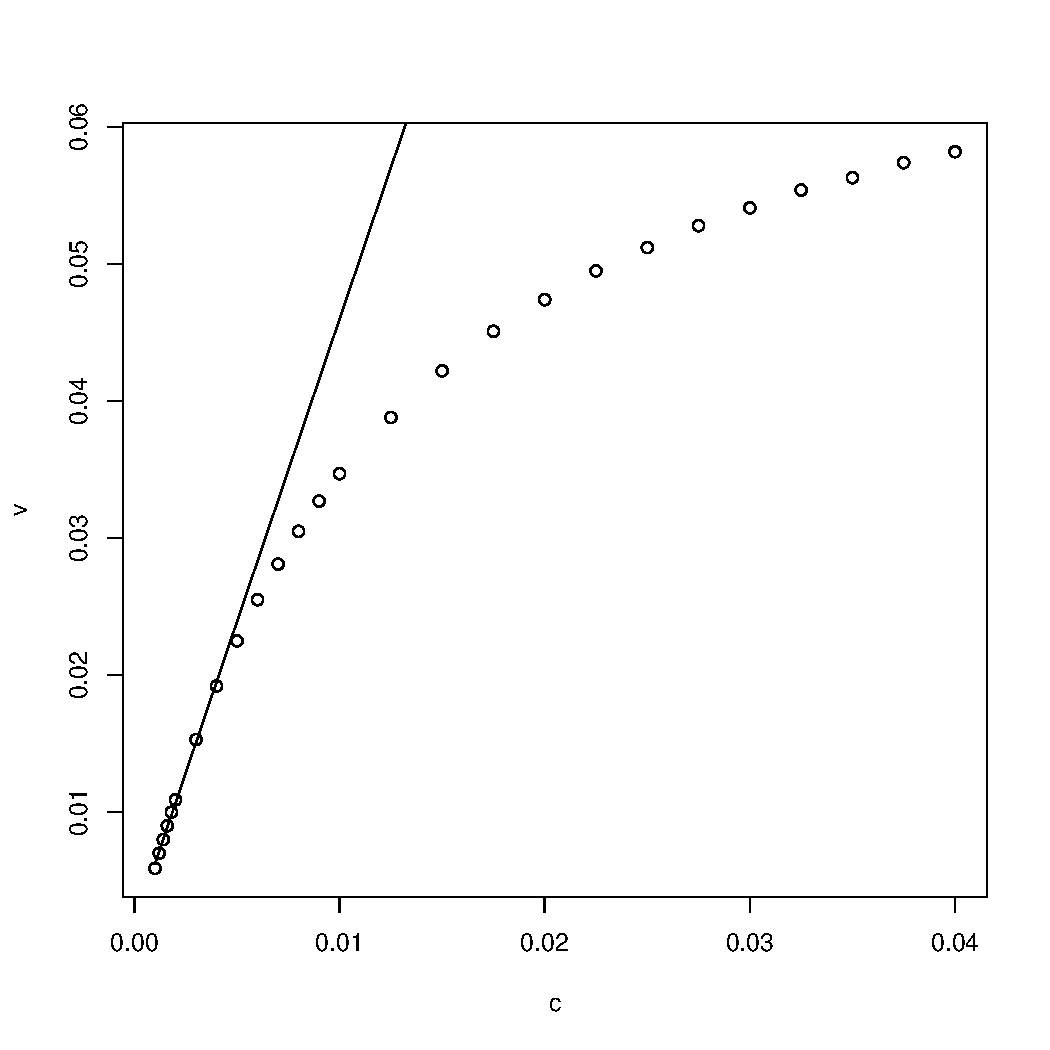
\includegraphics[width=\textwidth]{kemi2.pdf}

Jeg laver lineær regression på de første 8 punkter, dvs. dem der er under 0.02 på y-aksen. Jeg får
at hældningen er 4.417 så formlen bliver
$$v = 4.417\cdot [valin]^1$$
enheden på v skal i dette tilfælde være mol/s, og derfor skal k have enheden $s^-1$.
Så k bliver $4.417\ s^-1$

\end{document}
